\documentclass[a4paper,10pt]{article}
\usepackage[utf8]{inputenc}
\usepackage{pgfplots}
\pgfplotsset{compat=1.15}

\input{aux/tex/encabezado.tex}
\newif\ifen
\newif\ifes
\newcommand{\en}[1]{\ifen#1\fi}
\newcommand{\es}[1]{\ifes#1\fi}
\entrue

\title{Variational logistic regression}

\author{Gustavo Landfried}
\affil{\small Universidad de Buenos Aires. Facultad de Ciencias Exactas y Naturales. Departamento de Computaci\'on. Buenos Aires, Argentina}
\affil[]{Correspondencia: \url{gustavolandfried@gmail.com}}


\begin{document}

\maketitle

The dual 

\section{Local Variational Methods}

\en{The variational framework generally considered are ``global'' methods in the sense that it directly seeks an approximation to the full posterior distribution over all random variables.}
\es{}
%
\en{An alternative ``local'' approach involves finding bounds on functions over individual variables or groups of variables within a model.}
\es{}
%
\en{The convexity of the logarithm function played a key role in developing the lower bound in the global variational approach.}
\es{}
%
\en{Convexity also plays a central role in the local variational framework.}
\es{}

% Parrafo 

\en{Let us begin by considering a simple example,}
\es{}
%
\begin{equation}
f(x) = e^{-x} 
\end{equation}
%
\en{which is a convex function of $x$.}
\es{}
%
\en{Our goal is to approximate $f(x)$ by a simpler function, in particular a linear function of $x$.}
\es{}
%
\en{We can obtain the tangent line at a specific value of $x = \xi $, by making a first order Taylor expansion, $f(\xi) + f'(\xi)(x-\xi)$.}
\es{}
%
\begin{equation}
 y_{\xi}(x) = e^{-\xi} - e^{-\xi}(x-\xi)
\end{equation}
%
\begin{figure}[H]
\centering
\begin{tikzpicture}
  \draw[->] (-0.5, 0) -- (2, 0) node[right] {$x$};
  \draw[->] (0, -0.1) -- (0, 2) node[above] {$y$};
  \draw[scale=1, domain=-0.5:2, smooth, variable=\x, black!80] plot ({\x}, {e^(-\x)});
  \draw[scale=1, domain=-0.25:1.25, smooth, variable=\x, black!60] plot ({\x}, {e^(-0.5)-(e^(-0.5))*(\x-0.5)});
  \node at (0.5,{e^(-0.5)}) {\color{black!80}{\textbullet}};
  \end{tikzpicture}
\caption{}
\end{figure}
%
\en{so that $y_\xi(x) \leq f(x)$ with equality when $x = \xi$.}
%
\en{For consistency with subsequent discussion, let us define $\lambda_\xi = -e^{-\xi}$ so that}
%
\begin{equation}
\begin{split}
 y_\xi(x) & = - \lambda_\xi + \lambda_\xi (x + \log -\lambda_\xi) \\
 & = \lambda_\xi x - \lambda_\xi + \lambda_\xi \log -\lambda_\xi
 \end{split}
\end{equation}
%
\en{Different values of $\xi$ correspond to different tangent lines, and because all such lines are lower bounds on the function, we have $f(x_0) \geq y_\xi(x_0)$.}
%
\begin{equation}
\begin{split}
 0 & = \underset{\xi}{\text{arg min }} f(x_0) - y_\xi(x_0) \\
 - f(x_0) & = \underset{\xi}{\text{arg min }}  - y_\xi(x_0) \\
 f(x_0) & = \underset{\xi}{\text{arg max }}  y_\xi(x_0) \\
\end{split}
\end{equation}
%
\en{where we fix $x_0$ and optimize with respect to $\xi$.}
%
\begin{figure}[H]
\centering
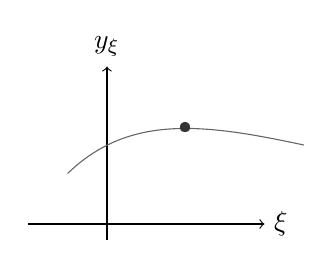
\begin{tikzpicture}
  \draw[->] (2*-0.5, 0) -- (2*1, 0) node[right] {$\xi$};
  \draw[->] (0, 2*-0.1) -- (0, 2*1) node[above] {$y_\xi$};
  \draw[scale=2, domain=-0.25:1.25, smooth, variable=\x, black!60] plot ({\x}, {e^(-\x)-(e^(-\x))*(0.5-\x)});
  \node at (2*0.5,{2*e^(-0.5)}) {\color{black!80}{\textbullet}};
  \end{tikzpicture}
\caption{}
\end{figure}
%
\en{We have succeeded in approximating the convex function $f(x_0)$ by a simpler, linear function $y_\xi(x_0)$.}
%
\en{The price we have paid is that we have introduced a variational parameter $\xi$, and to obtain the tightest bound we must optimize with respect to $\xi$.}
%
\begin{equation}
 f(x_0)  = \underset{\xi}{\text{arg max }}  \lambda_\xi x_0 - \underbrace{\lambda_\xi + \lambda_\xi \log -\lambda_\xi}_{\text{intercept }g(\lambda_\xi)} = \underset{\xi}{\text{arg max }} \lambda_\xi x_0 - g(\lambda_\xi)
\end{equation}
%
\en{Now, instead of fixing $x_0$ and varying $\xi$, we can consider a particular $\xi_0$ and then find the $x$ with minium distance between the tangent and the function.}
%
\begin{equation}
 g(\lambda_{\xi_0}) = \underset{x}{\text{arg min }} \lambda_{\xi_0} x - f(x) 
\end{equation}
%
\en{We see that the functions $f(x)$ and $g(\lambda_\xi)$ play a dual role.}

\vspace{0.3cm} % Parrafo 

\en{An important example, which arises frequently in pattern recognition, is the logistic sigmoid function defined by}
%
\begin{equation}
 \sigma(x) = \frac{1}{1 + e^{-x}}
\end{equation}
%
\en{As it stands this function is neither convex nor concave.}
%
\en{However, if we take the logarithm we obtain a function which is concave.}
%
\begin{equation}
 f(x) = \log \sigma(x) =  - \log(1 + e^{-x})
\end{equation}
%
\en{As is verified by finding the second derivative.}
%
\en{We begin by calculating the first derivative.}
%
\begin{equation}
 \frac{df}{dx} = (- \frac{1}{1 + e^{-x}}) \cdot(-e^{-x}) =  \frac{e^{-x}}{1 + e^{-x}} =\sigma(x) e^{-x}
\end{equation}
%
\en{Then we can obtain the second derivative.}
%
\begin{equation}
\begin{split}
 \frac{d^2f}{d^2x} & = \frac{-e^{-x}(1 + e^{-x}) - e^{-x}(-e^{-x})}{(1 + e^{-x})^2} \\
 & = \frac{-e^{-x} - e^{-2x} + e^{2x}}{(1 + e^{-x})^2} =  \frac{-e^{-x}}{(1 + e^{-x})^2} = - \sigma(x)^2 e^{-x} < 0
 \end{split}
\end{equation}
%
\en{Therefore, the log logistic sigmoid function $f(x)$ is concave, so we can find the upper bound on the log sigmoid.}
%
\begin{equation}
 y_\xi(x) = -\log (1 + e^{-\xi}) + \frac{e^{-\xi}}{1 + e^{-\xi}} (x - \xi)
\end{equation}
%
\en{We know that}
%
\begin{equation}
 \log \sigma(x) \leq y_\xi(x) 
\end{equation}
%
\en{And taking the exponential, we obtain an upper bound on the logistic sigmoid itself.}
%
\begin{equation}
 \sigma(x) \leq e^{y_\xi(x)}
\end{equation}


\begin{figure}[H]
\centering
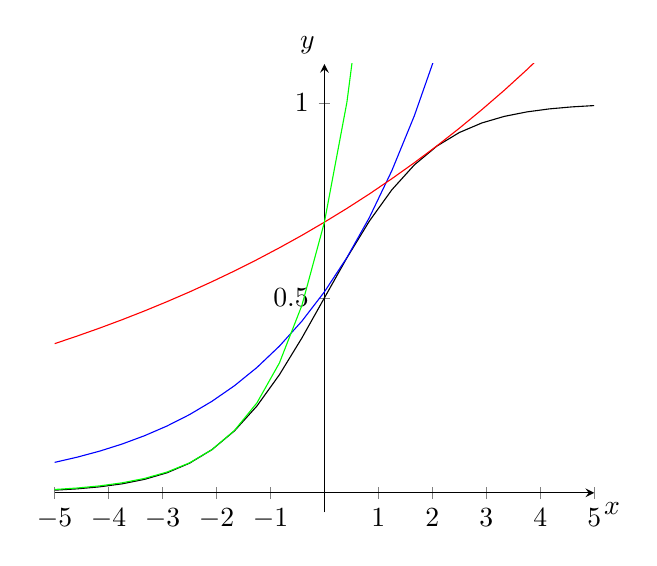
\begin{tikzpicture}
  \begin{axis}[
  axis x line=center,
  axis y line=center,
  xtick={-5,-4,...,5},
  ytick={0,0.5,1},
  xlabel={$x$},
  ylabel={$y$},
  xlabel style={below right},
  ylabel style={above left},
  xmin=-5,
  xmax=5,
  ymin=-0.05,
  ymax=1.1]
\addplot [mark=none,domain=-5:5] {1/(1+e^(-x)};
\addplot [mark=none,domain=-5:5, blue] {e^(-ln(1+e^(-0.5)) + (e^(-0.5)/(1+e^(-0.5)))*(x-0.5))};
\addplot [mark=none,domain=-5:5, red] {e^(-ln(1+e^(-2)) + (e^(-2)/(1+e^(-2)))*(x-2))};
\addplot [mark=none,domain=-5:5, green] {e^(-ln(1+e^(2)) + (e^(2)/(1+e^(2)))*(x+2))};
\end{axis}
\end{tikzpicture}
\caption{}
\end{figure}

\vspace{0.3cm} % Parrafo

\en{We can also obtain a lower bound on the sigmoid having the functional form of a Gaussian.}
%
\en{To do this we make transformations both of the input variable and of the function itself.}
%
\en{First we note that the function $\sigma(x)$ is a convex function of the variable $x^2$, as can again be verified by finding the second derivative or by insepction.}
%
\begin{figure}[H]
\centering
\scalebox{.7}{
\begin{tikzpicture}
  \begin{axis}[
  axis x line=center,
  axis y line=center,
  xtick={-5,-4,...,5},
  ytick={0,0.5,1},
  xlabel={$x$},
  ylabel={$y$},
  xlabel style={below right},
  ylabel style={above left},
  xmin=-5,
  xmax=5,
  ymin=0.45,
  ymax=1.1]
\addplot [mark=none,domain=-5:5] {1/(1+e^(-(x^2))};
\end{axis}
\end{tikzpicture}
}
\caption{}
\end{figure}
%
\en{Therefore $\log \sigma(x^2)$ also is convex.}
%
\en{If we decompose the log of the logistic function so that, we find a function that is concave,}
%
\begin{align}
 \log \sigma(x) & = - \log(1 + e^{-x}) = - \log(e^{-x/2} (e^{x/2} + e^{-x/2})) \\
 & = x/2 \underbrace{- \log(e^{x/2} + e^{-x/2})}_{f(x)} = x/2 + f(x)
\end{align}
%
\en{Where $f(x^2)$ is concave.}
%
\en{We compute the derivative of $f(x) = - \log(e^{x/2}+e^{-x/2})$}
%
\begin{equation}
\frac{df}{dx} = -\frac{1}{e^{x/2}+e^{-x/2}} \cdot \frac{1}{2} e^{x/2} -\frac{1}{2} e^{-x/2} = - \frac{1}{2} \frac{e^{x/2}-e^{-x/2}}{e^{x/2}+e^{-x/2}}
\end{equation}





\section{Lower bound de la funci\'on log\'istica}\label{sec:lower_bound}

\en{Here we shall make use of a Variational approximation based on local bounds, allowing the likelihood to be approximated by the exponential of a cuadratic form.}
\es{Aquí haremos uso de una aproximación variacional basada en acercamientos locales, permitiendo que la probabilidad sea aproximada por el exponencial de una forma cuadrática.}

\todo[inline]{Section 10.5 bishop}

The lower bound of the sigmoid then becomes
\begin{align}
 \sigma(x) \geq \sigma(\xi) \exp\left( \frac{x-\xi}{2} - \lambda(\xi)(x^2 - \xi^2) \right)
\end{align}

donde 
\begin{align}
 \lambda(\xi) = -\frac{1}{2\xi} \left( \sigma(\xi) - \frac{1}{2} \right)
\end{align}




\section{Distribuci\'on variacional a posteriori}

Likelihood
\begin{align*}
 p(t|\vm{w}) = \sigma(\vm{w}^T\bm{\phi})^t  (1-\sigma(\vm{w}^T\bm{\phi}))^{1-t}
\end{align*}

por independecia el joint likelihood
\begin{align*}
 p(\vm{t}|\vm{w}) & = \prod_{i=1}^N  p(t|\vm{w}) \\
 & = \prod_{i=1}^N  \sigma(\vm{w}^T\bm{\phi}_i)^t  (1-\sigma(\vm{w}^T\bm{\phi}_i))^{1-t}
\end{align*}

Predicci\'on a priori
\begin{align}
 p(\vm{t}) & = \int p(\vm{t}|\vm{w})p(\vm{w}) d\vm{w}  \\
 & = \int \left[ \prod_{i=1}^N p(t_i|\vm{w}) \right] p(\vm{w}) d\vm{w}
\end{align}

Para obtener el lower bound de $p(\vm{t})$ hacemos uso del resultado de la secci\'on~\ref{sec:lower_bound} que nos permite asegurar
\begin{align}
 \sigma(z) \geq \sigma()
\end{align}







\end{document}
